\subsubsection{Einführung in die Balkenbiegung}
Anhand der \textit{Balkentheorie nach Bernoulli} soll im Folgenden das mechanische Verhalten des Holms unter gegebenen Bedingungen ermittelt werden. Dazu werden einführend diese Theorie und andere Zusammenhänge kurz dargestellt.\\

\noindent Die Balkentheorie beschreibt elastische Längs- und Querverformungen eines Balkens beliebigen Querschnitts, resultierend durch angreifende Kräfte, Streckenlasten und Momente. Diese können durch Lager oder äußere angreifende Lasten in einen solchen Körper eingeleitet werden. Ergänzend sei angemerkt, dass es sich bei einem Balken um einen Körper handelt, dessen Länge sehr viel größere Werte als die der Breite und der Höhe besitzt. Durch die Lasten herrschen im Balken innere Normal- und Querkräfte und innere Momente $(N, Q, M)$. Mittels des Freischneidens können diese an beliebigen Stellen berechnet werden. Folgend ergeben sich Normal- (Zug, Druck) und Schubspannungen $(\sigma, \tau)$, die wiederum über das \textit{Hooke´sche Gesetz} zu Dehnungen und Verzerrungen $(\epsilon, \gamma)$ führen, sodass letztendlich anhand derer beschriebene Verformungen $(u, v, w)$ zu erkennen sind. Durch das hohe Verhältnis der Abmessungen zueinander werden Schubspannungen im Weiteren vernachlässigt \cite{item15}\cite{item16}\cite{item9}. \\

\noindent Für die Reaktionseigenschaften auf angreifende Lasten sind Materialkennwerte und die Geometrie des Balkens verantwortlich, welche mit der Biegesteifigkeit $EI$ repräsentiert werden. Gebildet wird sie durch den E-Modul $E$ und das Flächenträgheitsmoment $I$. Während Ersteres eine wichtige Eigenschaft eines Materials ist, ist Letzteres von der Querschnittsform abhängig. Neben der eigentlichen Form können ebenfalls Steiner-Anteile das Flächenträgheitsmoment erhöhen. Für die zu verwendenden Formeln wird auf das spätere Kapitel \ref{SP-Koord} verwiesen \cite{item16}.\\


\noindent Innerhalb des gebogenen Balkens gibt es stets eine neutrale Faser, die eine Linie bzw. Fläche ohne eine relative Längenänderung unter angreifenden Kräften und Momenten repräsentiert. Diese Linie wird auch Biegelinie genannt, für welche die vereinfachte \textit{Differentialgleichung des Biegebalkens}
\begin{equation}
	w^{''}=-\frac{M}{EI}
\end{equation}
aufgestellt wurde. Neben der Krümmung $w^{''}$ kann mittels Integration der Biegewinkel $w^{'}$ und die Absenkung $w$ bestimmt werden. Über Differentiationen werden auch äußere Momente, Kräfte und Streckenlasten in der Balkentheorie mit einbezogen. Durch Integrationskonstanten können geometrische Rand- und Übergangsbedingungen beachtet werden. Während in der neutralen Faser keine Normalspannungen auftreten, sind diese in den Randfasern maximal \cite{item16}\cite{item9}.\\

\noindent Es sei außerdem angemerkt, dass jederzeit Superpositions-Eigenschaften gelten. Dadurch können einerseits mehrere Balken in einem System betrachtet werden, andererseits aber auch Balken mit mehreren Belastungen in einzelne einfache Berechnungen überführt werden \cite{item16}.\\

\noindent Für die Berechnung einer Balkenbiegung kann nach folgendem Schema vorgegangen werden: Vorerst werden die notwendigen Lagerkräfte und -momente bestimmt. Wichtige Lagerarten bilden dabei das Festlager (ein rotatorischer Freiheitsgrad), das Loslager (ein rotatorischer und ein translatorischer Freiheitsgrad) und eine Einspannung (keine Freiheitsgrade), die Freiheitsgrade seien dabei auf den zweidimensionalen Fall bezogen. Anschließend wird der Balken bereichsweise an  Unstetigkeiten (z.B. Lager oder Krafteinleitungspunkte und ändernde Geometrien) geschnitten, um innere Kräfte am entstandenen positiven und negativen Schnittufer zu ermitteln. Dadurch lassen sich in diesen markanten Orten relevante Rand- und Übergangsbedingungen der Differentialgleichung des Biegebalkens bestimmen. Abschließend führen Integrationen und Differentiationen dieser Gleichung und deren Lösung  zur Absenkung, dem Biegewinkel, der Krümmung sowie innerem Kraft- bzw. Momentverlauf \cite{item16}\cite{item9}.


\subsubsection{Annahmen zur Modellierung}
Das Koordinatensystem des Flügels entspricht einem allgemeinen Flugzeug-Koordinatensystem, sodass die Flügellängskoordinate durch $y$ definiert ist. Der Koordinatenursprung ist im Lager A positioniert, da es keinen allgemeinen Flugzeugschwerpunkt gibt. \\

\noindent Zur Vereinfachung aller analytischen Berechnungen soll anfangs eine wichtige Annahme getroffen werden: Der Holm wird lediglich auf Biegung durch eine Querkraft und die Flügelschale nur auf Torsion durch ein resultierendes Torsionsmoment beansprucht. Diese Annahme kann getroffen werden, da die jeweiligen Belastungensarten auf das entsprechend andere Bauteil eine sehr kleine relative Auswirkung haben gegenüber dem gesamten Flügel als Baugruppe. Diese Annahme ist auch bei Segelflugzeugen, wie z.B. der SB 14 der \glqq Aademische[n] Fliegergruppe Braunschweig e.V.\grqq\: erfolgt und vom Luftfahrtbundesamt akzeptiert worden \cite{item21}.\\

\noindent Der Holm inklusive des Holmstummels wird für die Belastung durch eine Prüfkraft $F_{pruef}$ in negative z-Richtung als Biegebalken ausgelegt. Dafür ist er an zwei Stellen gelagert, am Lager $A$ und am Lager $B$. Die Lager entsprechen den Verstiftungen (siehe Bauteil U-Profil der Aufgabenstellung). Um eine Überbestimmung des Systems zu vermeiden, wird das Lager $B$ als Loslager angenommen. Die Querkraftbolzen werden nicht durch ein Lager, sondern durch eine zusätzlich angreifende Kraft $F_{Q}$ simuliert, da eine biegeweiche Wurzelrippe eine nicht definierbare, unbekannte Absenkung erlaubt.\\

\noindent Als Randbedingungen der Modellierung sind die Halbspannweite $s$ und die Absenkung $w$ (bezogen auf KOS) gegeben. Für die Absenkung $w$ soll eine Sicherheit $j=1,1$ gesetzt werden. Zwischen Lager $A$ und $B$ wird die Länge $l_{1}$ angenommen, zwischen Lager $B$ und der Wurzelrippe $C$ die Länge $l_{2}$. Die verbleibende Länge bis zur Flügelspitze, an der die Prüfkraft $F_{pruef}$ wirkt, wird $l_{3}$ bezeichnet. Die Halbspannweite $s$ wird, beginnend in der Mitte der Verstiftungen, bis zur Flügelspitze gemessen. Ausgehend von dem Holmstummelende bis zum Lager $A$ wird $l_{0}$ als Länge definiert. Diese Länge ist jedoch unerheblich für die Modellierung, sie wird erst für die Massenbestimmung benötigt.\\

\noindent Anhand der Randbedingungen und der Einspannvorrichtung für den Versuchsaufbau ergeben sich folgende Längen (ebenfalls in Abb. ~\ref{fig:Holmmodellierung}~ dargestellt): 
\begin{equation}
	s = 0,848 m
\end{equation}
\begin{equation}
	l_{0} = 0,03 m
\end{equation}
\begin{equation}
	l_{1} = 0,076 m
\end{equation}
\begin{equation}
	l_{2} = 0,037 m 
\end{equation}
\begin{equation}
	l_{3} = s - \frac{l_{1}}{2} - l_{2} = 0,773 m
\end{equation}
\begin{equation}
	w_{j=1,1} = \frac{1}{j} * w = \frac{1}{1,1} * 0,022 m = 0,02 m
\end{equation}
\begin{figure}
	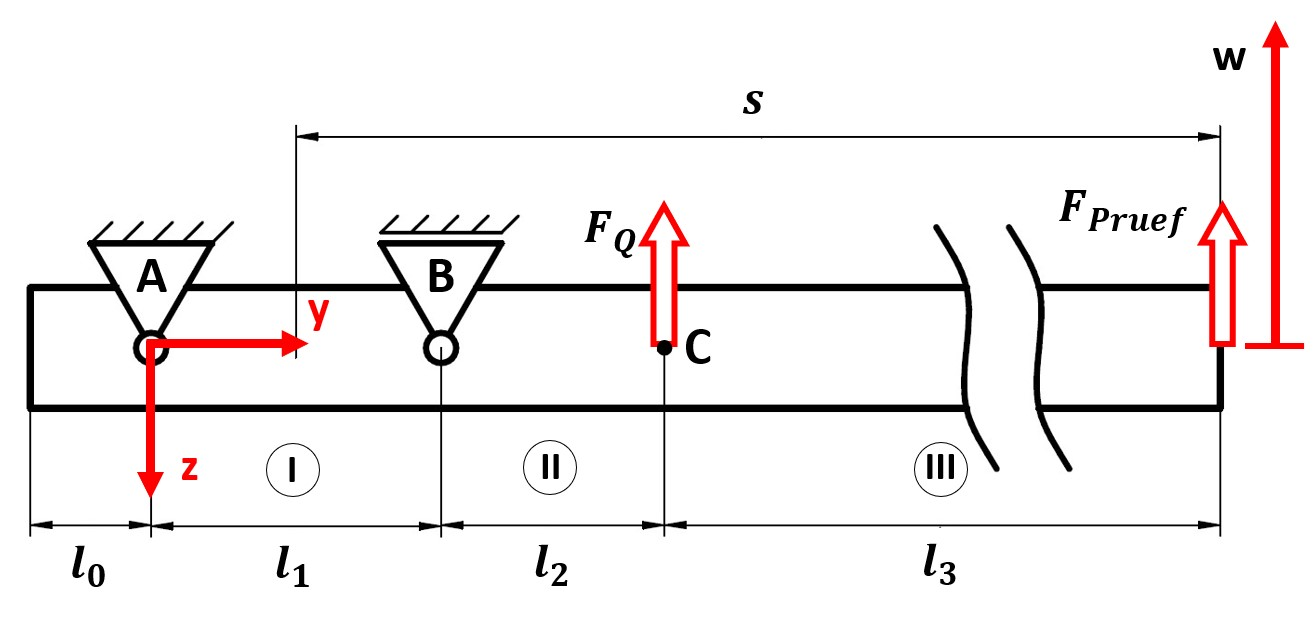
\includegraphics[width=1.0\textwidth]{Bilder/Balkenmodell2.jpg}
	\caption{Modellierung des Holms als Balken}
	\label{fig:Holmmodellierung}
\end{figure}

\subsubsection{Analytisches Lösen der Modellierung}
Um die Differentialgleichungen der Balkenbiegung lösen zu können, wird der Biegebalken vorerst in drei Teilbereiche $I$, $II$ und $III$ aufgeteilt, die sich von Lager $A$ zu $B$, von Lager $B$ zur Wurzelrippe $C$ und von dort aus bis zur Flügelspitze erstrecken. \\

\noindent Dadurch ergeben sich folgende zwölf Differentialgleichungen \cite{item16}:
\begin{equation} \label{eq:7}
	EI_{x}\cdot w_{I}^{''''}(y) = q_{I}(y)
\end{equation}
\begin{equation}\label{eq:8}
	EI_{x}\cdot w_{I}^{'''}(y) = q_{I}(y)\cdot y + R_{1} = -Q_{I}(y)
\end{equation}
\begin{equation}\label{eq:9}
	EI_{x}\cdot w_{I}^{''}(y) = \frac{q_{I}(y)}{2}\cdot y^{2} + R_{1}\cdot y + R_{2} = -M_{I}(y)
\end{equation}
\begin{equation}\label{eq:10}
	EI_{x}\cdot w_{I}^{'}(y) = \frac{q_{I}(y)}{6}\cdot y^{3} + \frac{R_{1}}{2}\cdot y^{2} + R_{2}\cdot y + R_{3} 
\end{equation}
\begin{equation}\label{eq:11}
	EI_{x}\cdot w_{I}(y) = \frac{q_{I}(y)}{24}\cdot y^{4} + \frac{R_{1}}{6}\cdot y^{3} + \frac{R_{2}}{2}\cdot y^{2} + R_{3}\cdot y + R_{4}
\end{equation}\\
\begin{equation}\label{eq:12}
	EI_{x}\cdot w_{II}^{''''}(y) = q_{II}(y)
\end{equation}
\begin{equation}\label{eq:13}
	EI_{x}\cdot w_{II}^{'''}(y) = q_{II}(y)\cdot y + R_{5} = -Q_{II}(y)
\end{equation}
\begin{equation}\label{eq:14}
	EI_{x}\cdot w_{II}^{''}(y) = \frac{q_{II}(y)}{2}\cdot y^{2} + R_{5}\cdot y + R_{6} = -M_{II}(y)
\end{equation}
\begin{equation}\label{eq:15}
	EI_{x}\cdot w_{II}^{'}(y) = \frac{q_{II}(y)}{6}\cdot y^{3} + \frac{R_{5}}{2}\cdot y^{2} + R_{6}\cdot y + R_{7} 
\end{equation}
\begin{equation}\label{eq:16}
	EI_{x}\cdot w_{II}(y) = \frac{q_{II}(y)}{24}\cdot y^{4} + \frac{R_{5}}{6}\cdot y^{3} + \frac{R_{6}}{2}\cdot y^{2} + R_{7}\cdot y + R_{8}
\end{equation}\\
\begin{equation}\label{eq:17}
	EI_{x}\cdot w_{III}^{''''}(y) = q_{III}(y)
\end{equation}
\begin{equation}\label{eq:18}
	EI_{x}\cdot w_{III}^{'''}(y) = q_{III}(y)\cdot y + R_{9} = -Q_{I}(y)
\end{equation}
\begin{equation}\label{eq:19}
	EI_{x}\cdot w_{III}^{''}(y) = \frac{q_{III}(y)}{2}\cdot y^{2} + R_{9}\cdot y + R_{10} = -M_{I}(y)
\end{equation}
\begin{equation}\label{eq:20}
	EI_{x}\cdot w_{III}^{'}(y) = \frac{q_{III}(y)}{6}\cdot y^{3} + \frac{R_{9}}{2}\cdot y^{2} + R_{10}\cdot y + R_{11} 
\end{equation}
\begin{equation}\label{eq:21}
	EI_{x}\cdot w_{III}(y) = \frac{q_{III}(y)}{24}\cdot y^{4} + \frac{R_{9}}{6}\cdot y^{3} + \frac{R_{10}}{2}\cdot y^{2} + R_{11}\cdot y + R_{12}
\end{equation}\\

\noindent Die Randbedingungen der Modellierung ergeben sich folgend nach gegebenen Definitionen von Lagern und angreifenden Kräften \cite{item16}: 
\begin{equation}\label{eq:22}
	w_{I}(y=0)=0
\end{equation}
\begin{equation}\label{eq:23}
	M_{I}(y=0)=0
\end{equation}\\
\begin{equation}\label{eq:24}
	w_{I}(y=l_{1}) = 0
\end{equation}
\begin{equation}\label{eq:25}
	w_{II}(y=l_{1}) = 0
\end{equation}
\begin{equation}\label{eq:26}
	w_{I}^{'}(y=l_{1}) = w_{II}^{'}(y=l_{1})
\end{equation}
\begin{equation}\label{eq:27}
	M_{I}(y=l_{1}) = M_{II}(y=l_{1})
\end{equation}\\
\begin{equation}\label{eq:28}
	w_{II}(y=l_{1}+l_{2}) = w_{III}(y=l_{1}+l_{2})
\end{equation}
\begin{equation}\label{eq:29}
	w_{II}^{'}(y=l_{1}+l_{2}) = w_{III}^{'}(y=l_{1}+l_{2})
\end{equation}
\begin{equation}\label{eq:30}
	M_{II}(y=l_{1}+l_{2}) = M_{III}(y=l_{1}+l_{2})
\end{equation}
\begin{equation}\label{eq:31}
	Q_{II}(y=l_{1}+l_{2}) = Q_{III}(y=l_{1}+l_{2})+F_{Q}
\end{equation}\\
\begin{equation}\label{eq:32}
	M_{III}(y=l_{1}+l_{2}+l_{3})=0
\end{equation}
\begin{equation}\label{eq:33}
	Q_{III}(y=l_{1}+l_{2}+l_{3})=F_{pruef}
\end{equation}
Zusätzlich wird angenommen, dass $q_{I}(y)=q_{II}(y)=q_{III}(y)=0$ gilt, da keine Streckenlast angreift. Unter anderem bildet die Schwerkraft der Erde eine Streckenlast, diese kann jedoch aufgrund ihres kleinen Einflusses auf die Absenkung gegenüber der Prüfkraft vernachlässigt werden. Ein weiteres Beispiel für eine Streckenlast bildet die Auftriebsverteilung eines Flügels während einer Anströmung. Jedoch wird genau auf diese im Versuchsstand verzichtet und durch die Prüfkraft repräsentiert.\\

\noindent Als Lösung dieser Differentialgleichungen lässt sich die Querkraft $Q(y)$, das Moment $M(y)$ und die Biegelinie $w(y)$ ermitteln:\\

\begin{equation}\label{eq:34}
	Q(y,F_{pruef},F_{Q},EI_{x})=\left\{\begin{array}{ll}
		F_{pruef}\cdot \frac{l_{2}+l_{3}}{l_{1}}-F_{Q}\cdot \frac{l_{2}}{l_{1}}&,y\epsilon (0,l_{1})\\
		F_{pruef}+F_{Q}&,y\epsilon (l_{1}, l_{1}+l_{2})\\
		F_{pruef}&,y\epsilon (l_{1}+l_{2}, l_{1}+l_{2}+l_{3})
	\end{array}\right.
\end{equation}\\
\begin{equation}\label{eq:35}
	M(y,F_{pruef},F_{Q},EI_{x})=\left\{\begin{array}{ll}
		(-F_{pruef}\cdot \frac{l_{2}+l_{3}}{l_{1}}-F_{Q}\cdot \frac{l_{2}}{l_{1}})\cdot y&,y\epsilon (0,l_{1})\\
		F_{pruef}\cdot (y-l_{1}+l_{2}+l_{3})+F_{Q}\cdot (y-l_{1}+l_{2})&,y\epsilon (l_{1}, l_{1}+l_{2})\\
		F_{pruef}\cdot (y-l_{1}+l_{2}+l_{3})&,y\epsilon (l_{1}+l_{2}, l_{1}+l_{2}+l_{3})
	\end{array}\right.
\end{equation}\\
\begin{equation}\label{eq:36}
	w(y,F_{pruef},F_{Q},EI_{x})=\left\{\begin{array}{ll}
		\frac{1}{EI_{x}}\cdot\frac{1}{6}\cdot\biggl((F_{pruef}\cdot \frac{l_{2}+l_{3}}{l_{1}}-F_{Q}\cdot \frac{l_{2}}{l_{1}})\cdot y^{3}-\Bigl((l_{2}+l_{3})\cdot l_{1}\cdot F_{pruef}\\-l_{1}\cdot l_{2}\cdot F_{Q}\Bigl)\cdot y \biggr)\:,y\epsilon (0,l_{1})&\\
		\frac{1}{EI_{x}}\cdot\biggl(\frac{(-F_{pruef}-F_{Q})}{6}\cdot y^{3} + \frac{F_{pruef}\cdot (l_{1}+l_{2}+l_{3})+F_{Q}\cdot (l_{1}+L_{2})}{2}\cdot y^{2}\\ + \Bigl(F_{pruef}\cdot(-\frac{1}{2}\cdot l_{1}^{2}-\frac{2}{3}\cdot l_{1}\cdot l_{2}-\frac{2}{3}\cdot l_{1}\cdot l_{3})+ F_{Q}\cdot(-\frac{1}{2}l_{1}^{2}-\frac{2}{3}\cdot l_{1}\cdot l_{2})\Bigr)\cdot y \\+ F_{pruef}\cdot\frac{1}{6}\cdot(l_{1}^{3}+l_{1}^{2}\cdot l_{2}+l_{1}^{2}\cdot l_{3}) + F_{Q}\cdot\frac{1}{6}\cdot(l_{1}^{3}+l_{1}^{2}\cdot l_{2})\biggr)&\\,y\epsilon (l_{1}, l_{1}+l_{2})\\
		\frac{1}{EI_{x}}\cdot\biggl(-\frac{F_{pruef}}{6}\cdot y^{3} + \frac{ F_{pruef}\cdot (l_{1}+l_{2}+l_{3})}{2}\cdot y^{2} + \Bigl(F_{pruef} \\
		\cdot(-\frac{1}{2}\cdot l_{1}^{2} -\frac{2}{3}\cdot l_{1}\cdot l_{2}-\frac{2}{3}\cdot l_{1}\cdot l_{3}) + F_{Q}\cdot(\frac{1}{2}\cdot l_{2}^{2}+\frac{1}{2}\cdot l_{1}\cdot l_{2})\Bigr)\cdot y \\ +F_{pruef}\cdot\frac{1}{6}\cdot(l_{1}^{3}+l_{1}^{2}\cdot l_{2}+l_{1}^{2}\cdot l_{3}) + F_{Q}\cdot(-\frac{1}{6}\cdot l_{2}^{3}-\frac{1}{3}\cdot l_{1}^{2}\cdot l_{2}-\frac{1}{2}\cdot l_{2}^{2}\cdot l_{1})\biggr)&\\,y\epsilon (l_{1}+l_{2}, l_{1}+l_{2}+l_{3})
	\end{array}\right.
\end{equation}\\
Die Herleitung der Lösung kann im Kapitel \ref{Lösung} nachvollzogen werden.\\

\noindent Um nun für die später geforderte Biegesteifigkeit $EI_{x}$ ein Ergebnis zu erhalten, wird die Gleichung $w(y,F_{pruef},F_{Q}, EI_{x})$ nach $EI_{x}(y,F_{pruef},F_{Q},w)$ umgestellt. Die eingesetzten Werte ergeben sich aus der Auslegung auf Steifigkeit. Über die Wurzelrippe werden Kräfte des Holms in die Querkraftbolzen abgesetzt. Aufgrund der biegeweichen Wurzelrippe als Verbindungselement zwischen Holm und den Querkraftbolzen darf die Absenkung des Holms dort nicht mit null angenommen werden. Vereinfacht wird definiert, dass die eingeleitete Prüfkraft $F_{pruef}$ an den Querkraftbolzen um ihren Betrag abgesetzt wird, wie es tatsächlich an einem Flugzeugrumpf geschehen würde. Dieses entspricht sehr wahrscheinlich jedoch nicht der tatsächlichen Kraftaufnahme im Versuchsaufbau.
\begin{equation}
	\begin{array}{l}
		EI_{x}(0.886m, 100N, -100N, 0.02m)= \\
		\frac{1}{w}\cdot\biggl(-\frac{F_{pruef}}{6}\cdot y^{3} + \frac{ F_{pruef}\cdot (l_{1}+l_{2}+l_{3})}{2}\cdot y^{2} + \Bigl(F_{pruef}\cdot(-\frac{1}{2}\cdot l_{1}^{2} -\frac{2}{3}\cdot l_{1}\cdot l_{2}-\frac{2}{3}\cdot l_{1}\cdot l_{3}) \\ +F_{Q}\cdot(\frac{1}{2}\cdot l_{2}^{2}+\frac{1}{2}\cdot l_{1}\cdot l_{2})\Bigr)\cdot y + F_{pruef}\cdot\frac{1}{6}\cdot(l_{1}^{3}+l_{1}^{2}\cdot l_{2}+l_{1}^{2}\cdot l_{3}) + F_{Q}\cdot(-\frac{1}{6}\cdot l_{2}^{3}-\frac{1}{3}\cdot l_{1}^{2}\cdot l_{2}-\frac{1}{2}\cdot l_{2}^{2}\cdot l_{1})\biggr)\\
		=962,552Nm^{2}
	\end{array}
\end{equation}

\subsubsection{Analyse der Modellierung}
In Abb. ~\ref{fig:Steifigkeitsauslegung} werden die Querkraftverläufe $Q(y,F_{pruef},F_{Q},EI_{x})$ als innere Schnittkraft, der Momentenverlauf $M(y,F_{pruef},F_{Q},EI_{x})$ als inneres Schnittmoment und die Biegelinie $w(y,F_{pruef},F_{Q},\\EI_{x})$ für den Nachweis der Steifigkeit graphisch dargestellt, über die gesamte Holmlänge und in einem vergrößerten Ausschnitt im Bereich der Lager. \\

\begin{figure}
	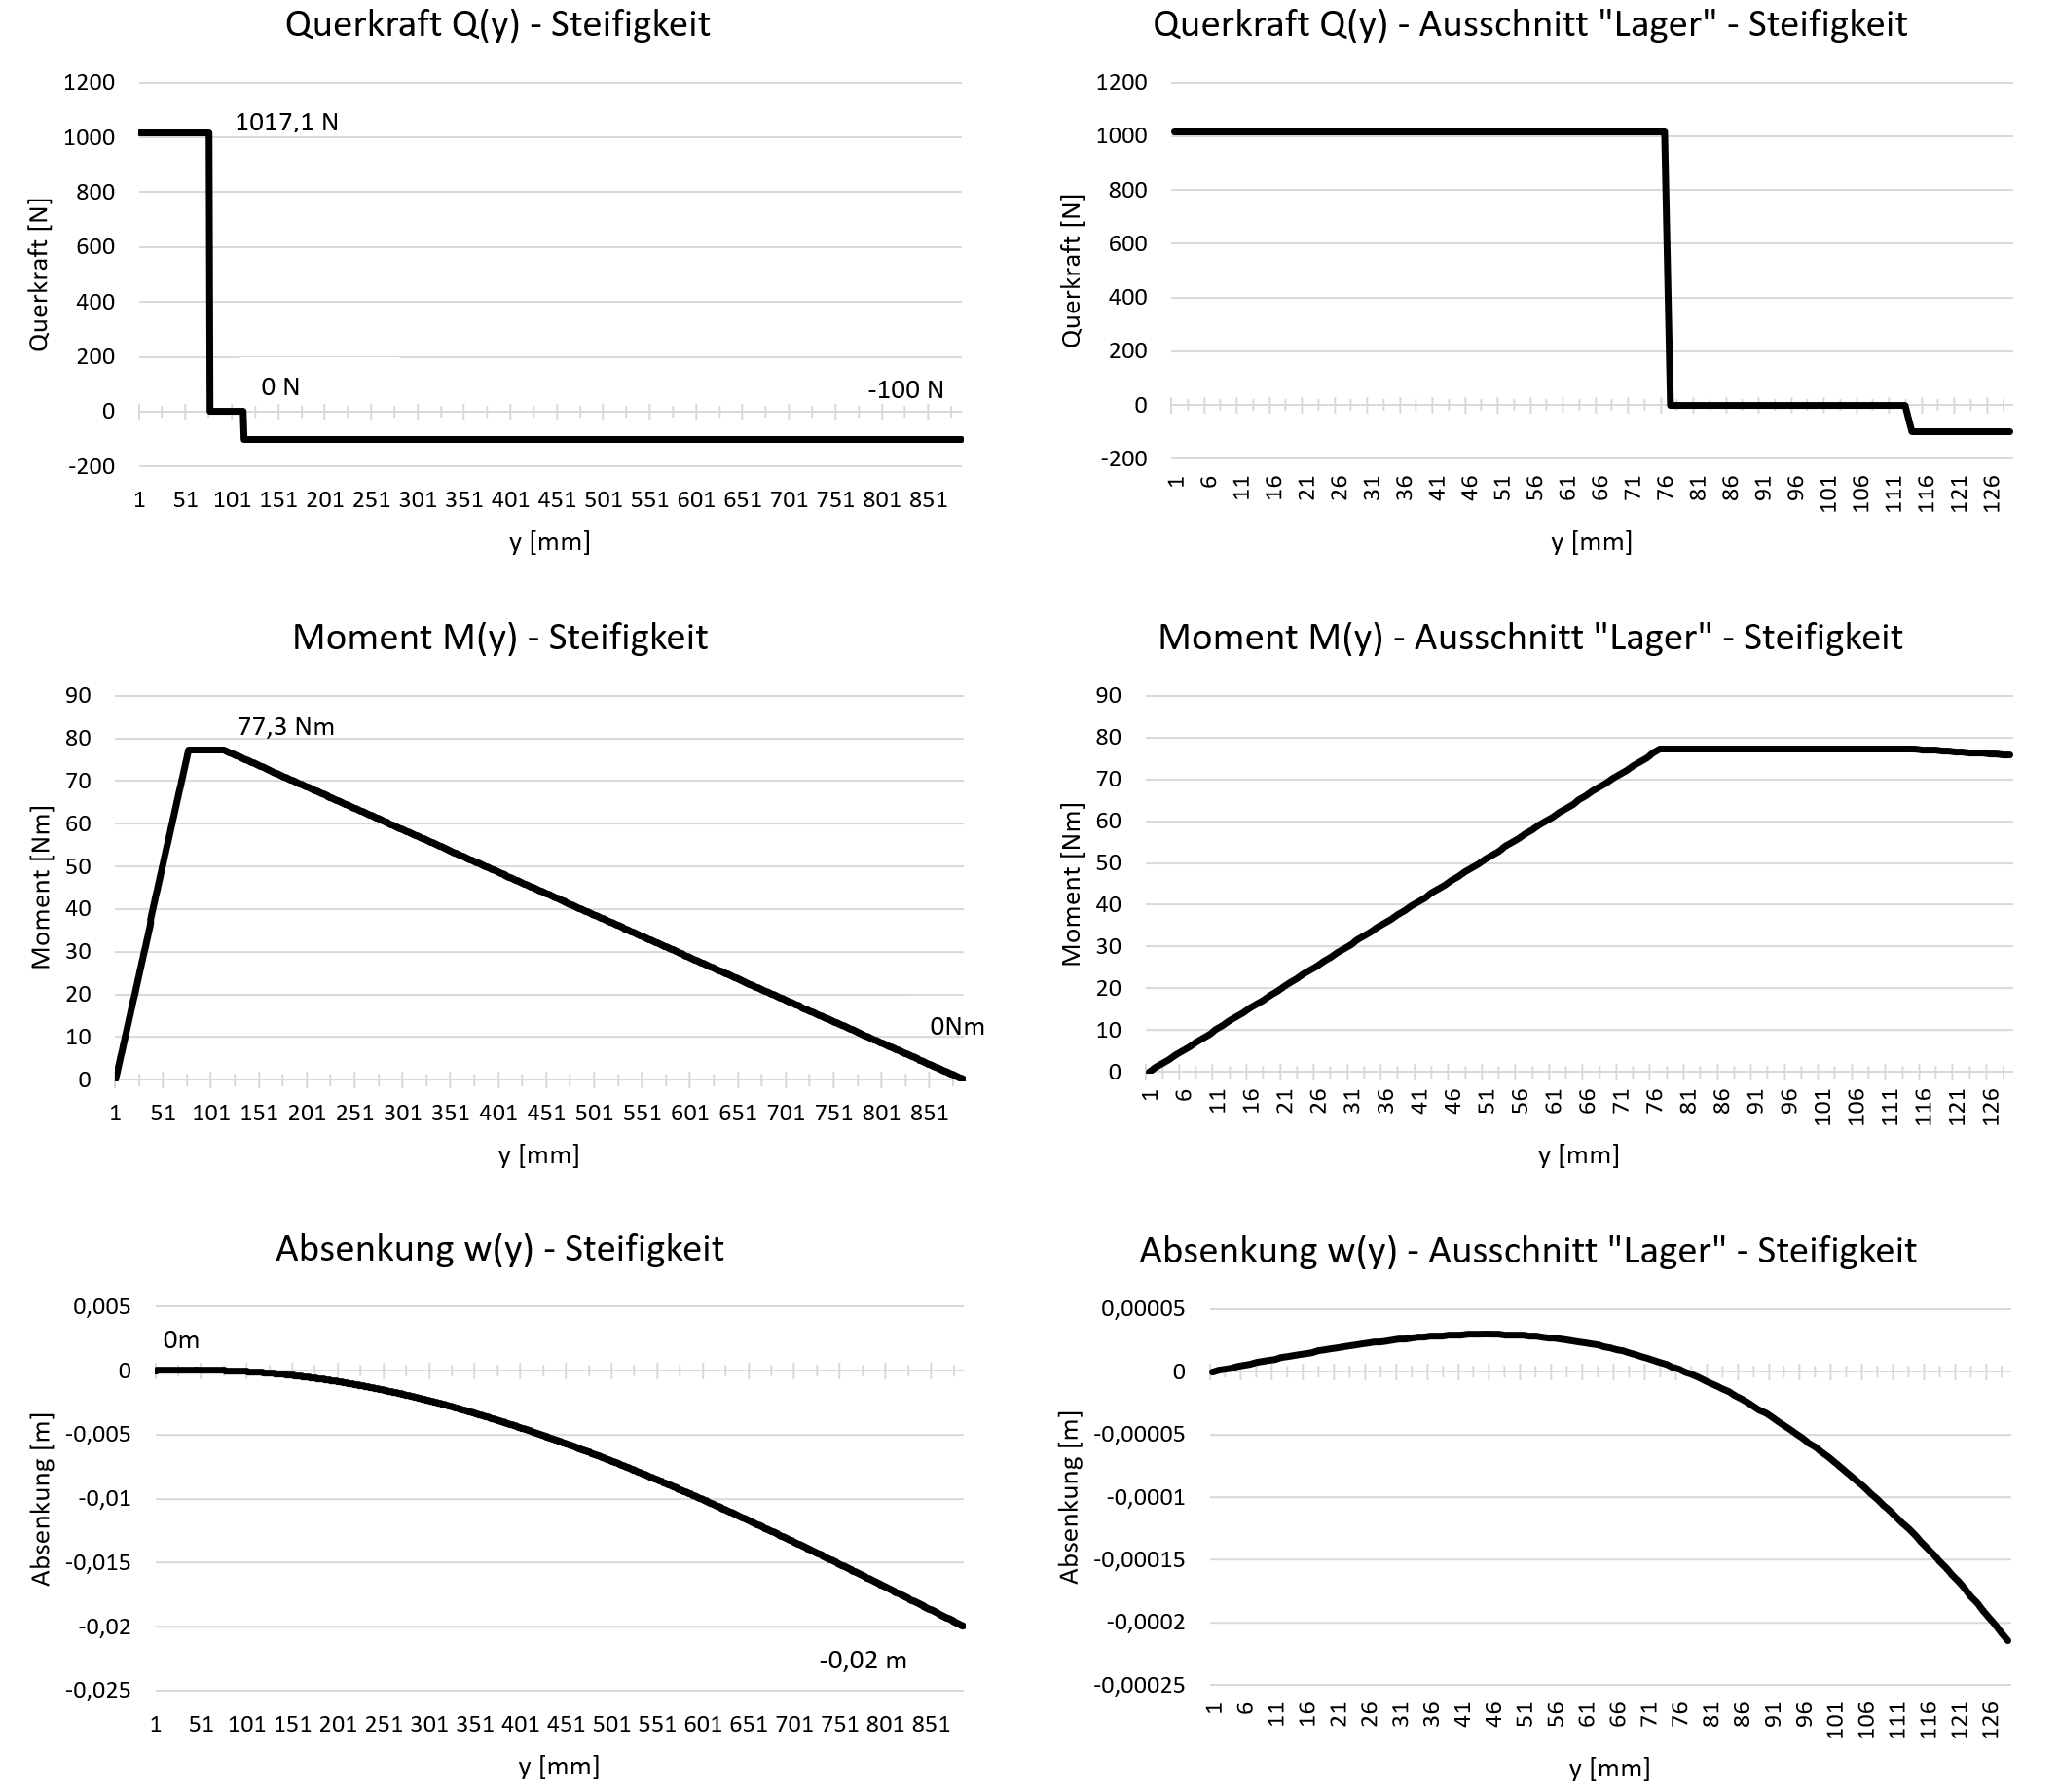
\includegraphics[width=1.0\textwidth]{Bilder/Grafiken Steifigkeit.png}
	\caption{Kraft-, Moment- und Absenkungsverlauf der Steifigkeitsauslegung des Holms}
	\label{fig:Steifigkeitsauslegung}
\end{figure}

\noindent Jedoch werden nicht bei dem Nachweis der Steifigkeit, sondern bei dem Nachweis der Festigkeit das maximale Schnittmoment und die maximale Schnittkraft erreicht. Bei diesem Nachweis beträgt die Prüfkraft $F_{pruef} = 500N$ und somit auch $|F_{Q}| = 500N$. Diese Kraft wird bei der Berechnung von $EI_{x}$ nicht beachtet, da bei dem Nachweis der Festigkeit die Absenkung $w$ kein Rolle spielt. In Abb. ~\ref{fig:Festigkeitsauslegung} werden die genannten Verläufe nun für den Festigkeitsnachweis dargestellt.
\begin{figure}
	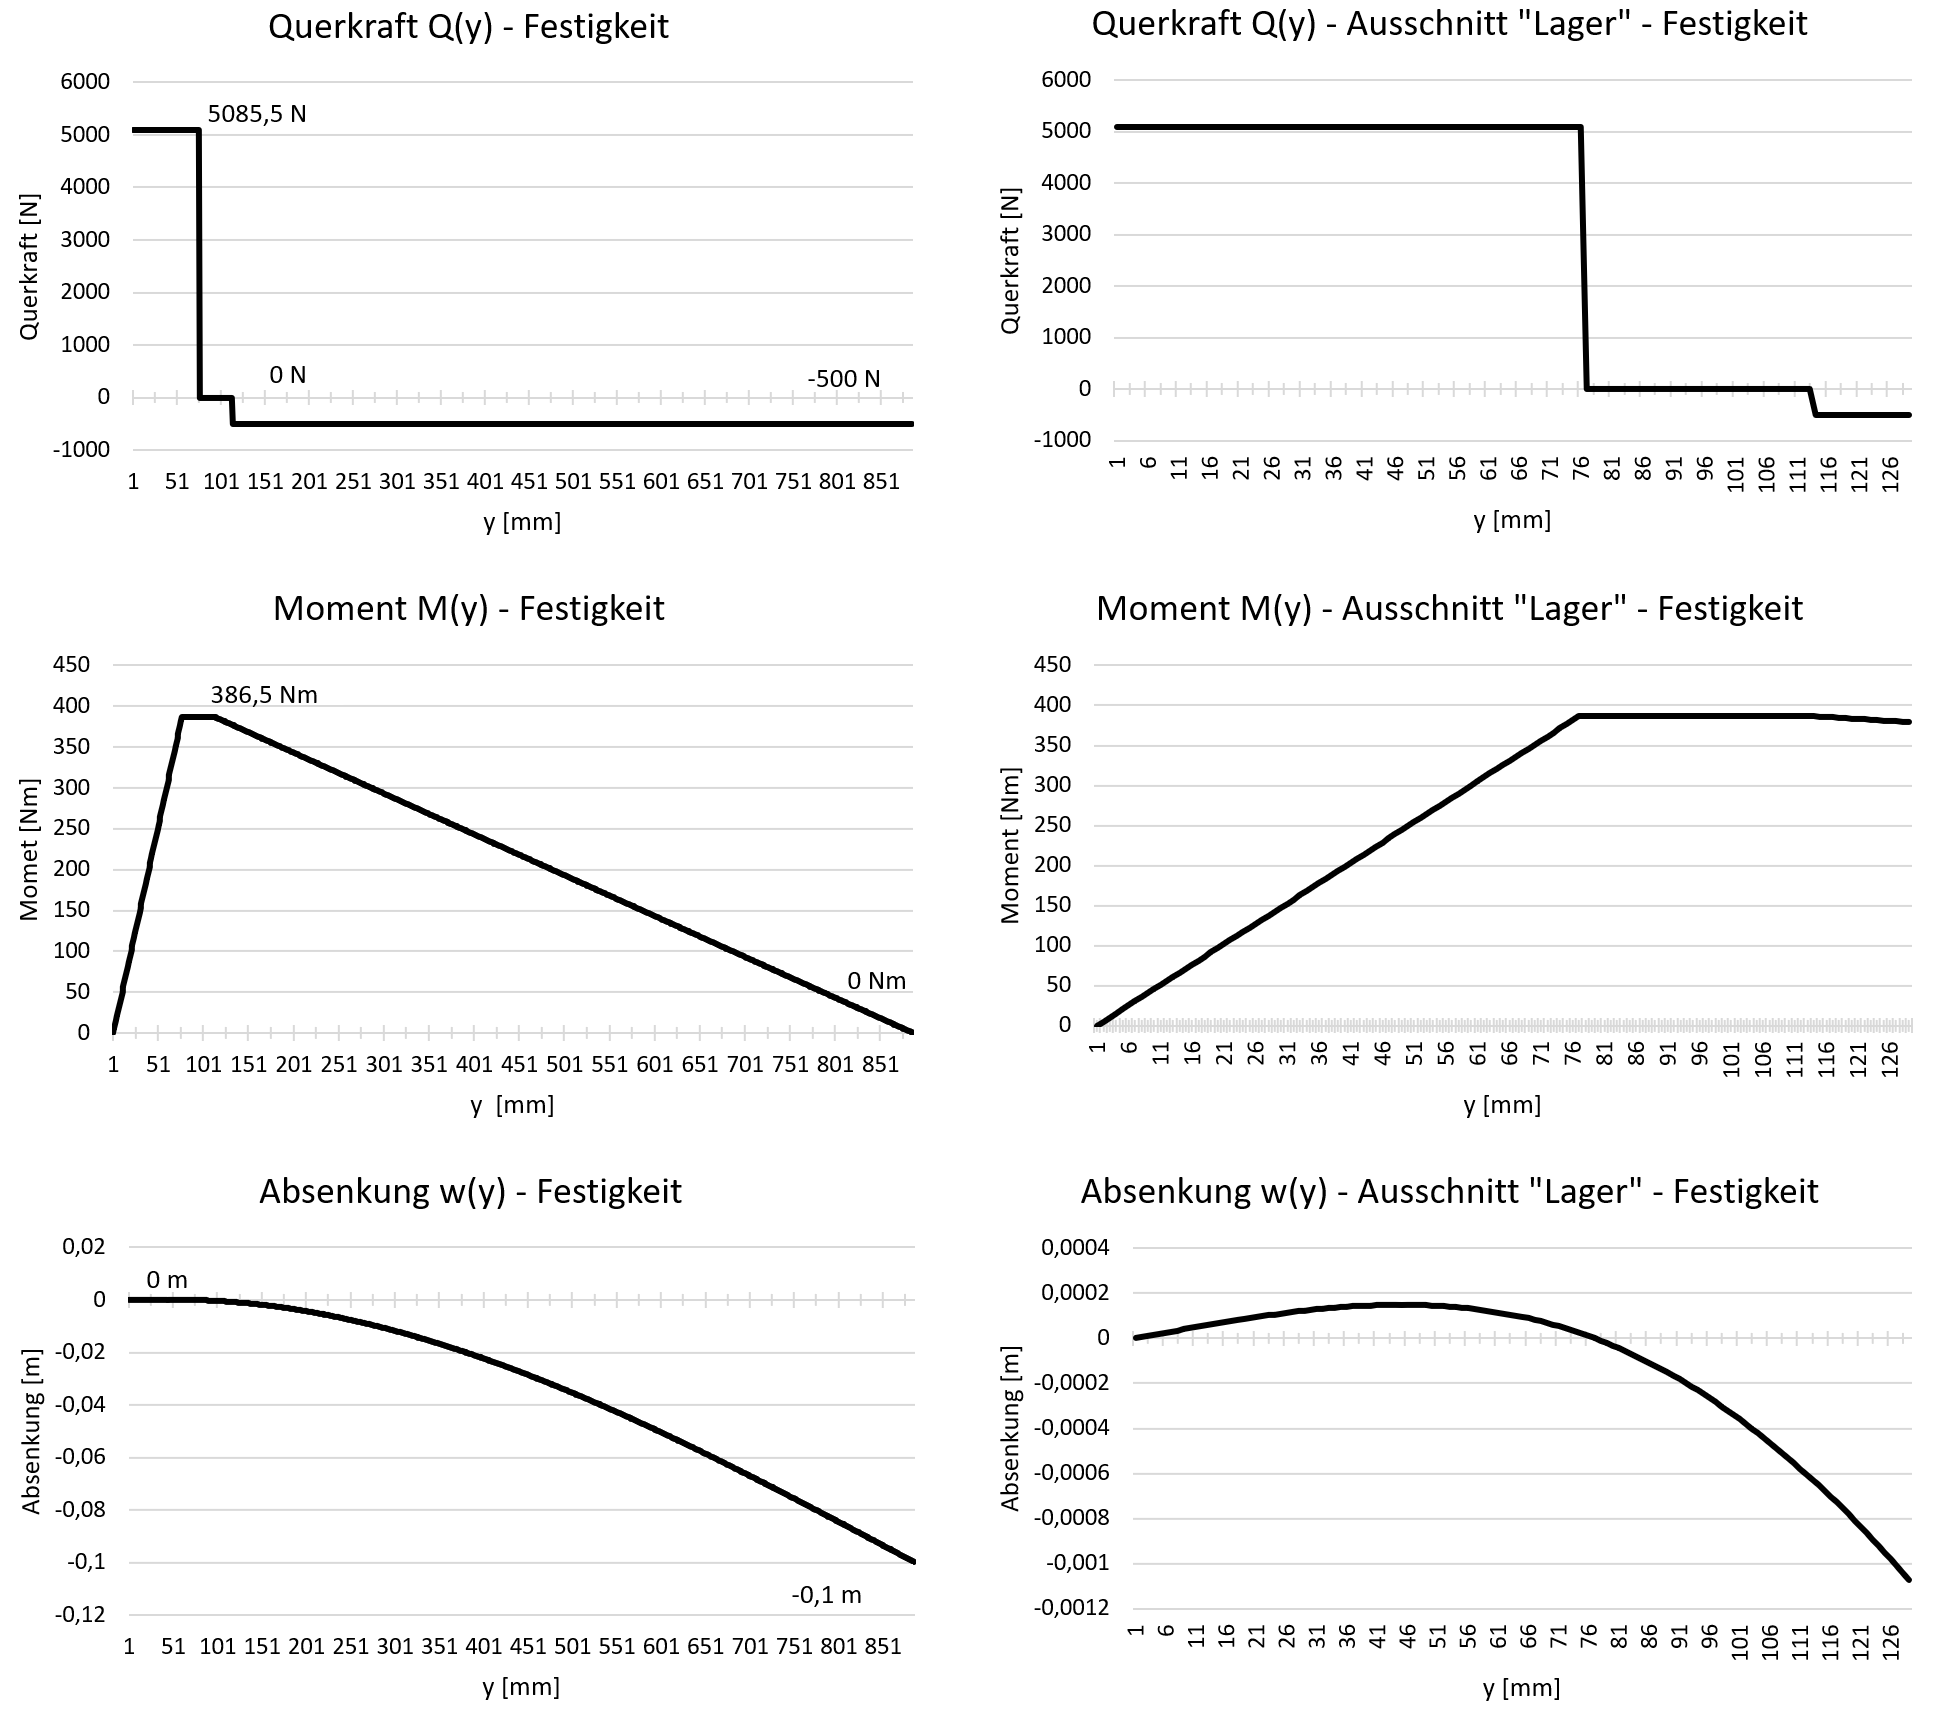
\includegraphics[width=1.0\textwidth]{Bilder/Grafiken Festigkeit.png}
	\caption{Kraft-, Moment- und Absenkungsverlauf der Festigkeitsauslegung des Holms}
	\label{fig:Festigkeitsauslegung}
\end{figure}

